% !TeX root = ../Book1.tex
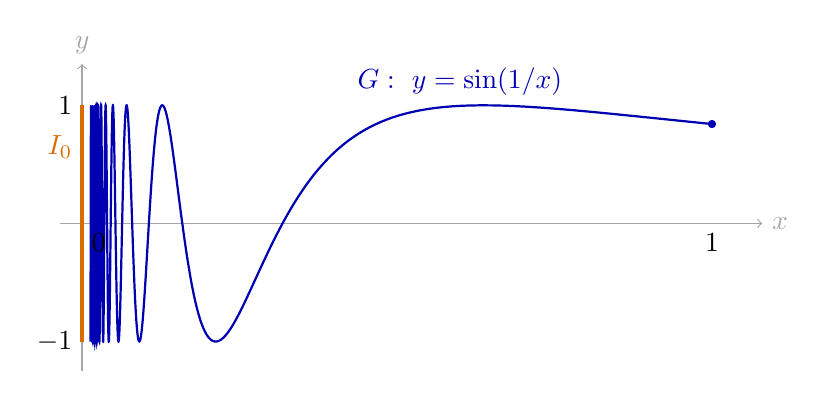
\begin{tikzpicture}[x=8cm,y=1.5cm]
	\draw[->,gray!70] (-0.035,0)--(1.08,0) node[right] {\(x\)};
	\draw[->,gray!70] (0,-1.25)--(0,1.35) node[above] {\(y\)};
	\draw[very thick,orange!85!black] (0,-1)--(0,1);
	\draw[blue!70!black,thick,domain=1:75,samples=1800,variable=\t] plot ({1/\t},{sin(\t r)});
	\fill[blue!70!black] (1,{sin(1 r)}) circle(1.5pt);
	\node[orange!85!black,left] at (0,0.65) {\(I_0\)};
	\node[blue!70!black] at (0.6,1.2) {\(G:\ y=\sin(1/x)\)};
	\node[below] at (1,0) {\(1\)};
	\node[left] at (0,-1) {\(-1\)};
	\node[left] at (0,1) {\(1\)};
	\node[below right] at (0,0) {\(0\)};
\end{tikzpicture}
